% PAKETE UND DOKUMENTKONFIGURATION
\documentclass[11pt, a4paper]{article}

% Encoding für Umlaute
\usepackage[utf8]{inputenc}
\usepackage[T1]{fontenc}

% Silbentrennung
\usepackage[ngerman]{babel}

% erweiterte Matheumgebungen und Formelnummer mit Sectionnummer
\usepackage{amsmath}
\numberwithin{equation}{section}

% Braket Notation
\usepackage{braket}
\usepackage{isotope}
\usepackage{mhchem}

% zusätzliche mathematische Schriftarten
\usepackage{amsfonts}

% verschiedene mathematische Symbole
\usepackage{amssymb}

% Einheiten setzen z.B. \SI{10}{\kilo\gram\meter\per\second\squared}
% Fehler: \SI{10 +- 0,2e-4}{\metre}
\usepackage{siunitx}
\sisetup{
  output-decimal-marker={,},
  separate-uncertainty
}

% Einheitendefinitionen
\DeclareSIUnit{\skt}{Skt.}
\DeclareSIUnit{\gauss}{G}
\DeclareSIUnit{\division}{div.}

% Operatordefinitionen
\DeclareMathOperator{\erf}{erf}

% Randbreiten
\usepackage[left=3.5cm,right=3.5cm,top=3cm,bottom=3cm,twoside]{geometry}

% Bilder einfügen
\usepackage{graphicx}

% Verweise innerhalb des Dokuments
\usepackage{hyperref}
\hypersetup{
	colorlinks = true,
	allcolors = {black}
}

% bessere Tabellenlayouts
\usepackage{booktabs}
\usepackage{multirow}
\usepackage{multicol}

% Seitenlayout (Kopfzeile)
\usepackage{fancyhdr}

% Float Barriers
\usepackage{placeins}

% Pakete für gedrehte Subfigures
\usepackage{caption}
\usepackage{subcaption}
\usepackage{rotating}

% Paket für textumflossene Abbildungen und Tabellen
\usepackage{wrapfig}

\usepackage{float}

% Caption-Setup
\captionsetup{font={small}}
\renewcommand{\thefigure}{\thesection.\arabic{figure}}
\renewcommand{\thesubfigure}{\alph{subfigure}}
\renewcommand{\thetable}{\thesection.\arabic{table}}
\renewcommand{\thesubtable}{\alph{subtable}}

% Manuelle Silbentrennung
\hyphenation{Sig-nal-ver-hal-ten Szin-til-la-tions-de-tek-tors}

% Tiefe des Inhaltsverzeichnisses (Level: 1 sections, 2 subsections,
% 3 subsubsections)
\setcounter{tocdepth}{3}

% FANCYHDR SETUP
\pagestyle{fancy}
\fancyhead[EL,OR]{\thepage}
\fancyhead[ER]{\leftmark}
\fancyhead[OL]{\rightmark}

\renewcommand{\sectionmark}[1]{
\markboth{\thesection{} #1}{\thesection{} #1}
}
\renewcommand{\subsectionmark}[1]{
\markright{\thesubsection{} #1}
}

\newcommand{\ptt}{Peak-to-Total-Verhältnis}
\newcommand{\co}{\isotope[60]{Co}}
\newcommand{\cs}{\isotope[137]{Cs}}
\newcommand{\eu}{\isotope[152]{Eu}}

% DOKUMENTINFORMATIONEN
\title{P529 \\ Dosimetrie und Abschirmung}

\author{Christopher Deutsch\footnote{christopher.deutsch@uni-bonn.de} \and Christian Bespin\footnote{christian.bespin@uni-bonn.de}}

\date{\today}

\begin{document}

\begin{titlepage}

\maketitle

% DURCHFÜHRUNGSDATUM UND TUTOR
\begin{center}
\begin{tabular}{l r}
Durchführung: & 27./28. April 2015 \\
Gruppe: & $\alpha$ 6 \\
Tutor: & Christian Hammann
\end{tabular}
\end{center}

% ZUSAMMENFASSUNG
\begin{abstract}
\noindent
\end{abstract}

\end{titlepage}

% INHALTSVERZEICHNIS
\tableofcontents
% Neue Seite nach TOC
\newpage

% INHALT VERSUCHSPROTOKOLL

\section{Einführung}

\section{Theorie}
\subsection{Röntgenstrahlung}
Als Röntgenstrahlung wird der Teil des elektromagnetischen Spektrums mit Photon-Energien zwischen \SI{100}{\electronvolt} und \SI{100}{\kilo\electronvolt} bezeichnet, wobei diese Grenzen nicht scharf sind und deshalb oft hinsichtlich der Strahlungsquelle eine Einordnung vollzogen wird.

\subsubsection{Erzeugung}
\label{sec:röntgenerzeugung}
Es gibt zwei typische Erzeugungsmethoden von Röntgenstrahlung, welche auf dem Beschuss eines \emph{Targets} mit einem hochenergetischen Elektronenstrahl bestehen.
Die beiden Strahlungsarten, welche in der Praxis oft zusammen auftreten, sind:
\begin{itemize}
	\item \textbf{Bremsstrahlung:} Die bei der Streuung der geladenen Elektronen an den Kernen des Targets vollzogene Geschwindigkeitsänderung des Elektrons, führt zur Emission eines Photons.
	Das so entstandene Spektrum ist kontinuierlich, wobei die maximale Photonenenergie gegeben ist durch die kinetische Energie der einfallenden Elektronen, welche durch deren Beschleunigungsspannung $U$ gegeben ist.
	Überträgt das Elektron seine gesamte Energie auf ein einzelnes Photon:
	\begin{align}
	&E_\mathrm{kin. e^-} = h \cdot \nu_\mathrm{max} = \frac{hc}{\lambda_\mathrm{min}}
	\end{align}
	so ist diese Grenze gegeben durch das \textbf{Duane-Hunt-Gesetz}
	\begin{align}
	\lambda_\mathrm{min} = \frac{h c}{e U}
	\end{align}
	Eine Quelle für reine Bremsstrahlung sind Synchrotronstrahlungsquellen.
	
	\item \textbf{charakteristische Strahlung:} Die einfallende hochenergetische Elektronenstrahlung ionisiert ein Elektron der inneren Schale eines Targetatoms.
	Dadurch entsteht ein freier Zustand, welcher durch ein Elektron einer weiter äußeren Schale eingenommen werden kann.
	Durch den Übergang wird ein Photon emittiert, dessen Energie gleich der Energiedifferenz der beiden Zustände ist.
	Aufgrund dieser Abhängigkeit von der elektronisches Struktur des Targetatoms, ist das emittierte, diskrete Spektrum charakteristisch für das verwendete (Target)-Material.
	Außerdem weist das emittierte Spektrum die Aufspaltung der Energieniveaus aufgrund von Fein- und Hyperfeinstruktur auf.
\end{itemize}
In der Praxis treten beide Effekte bei der Erzeugung von Röntgenstrahlen in sogenannten Röntgenröhren auf, wie in Abbildung \ref{fig:spektrum} zu sehen ist.
\begin{figure}[h]
	\centering
	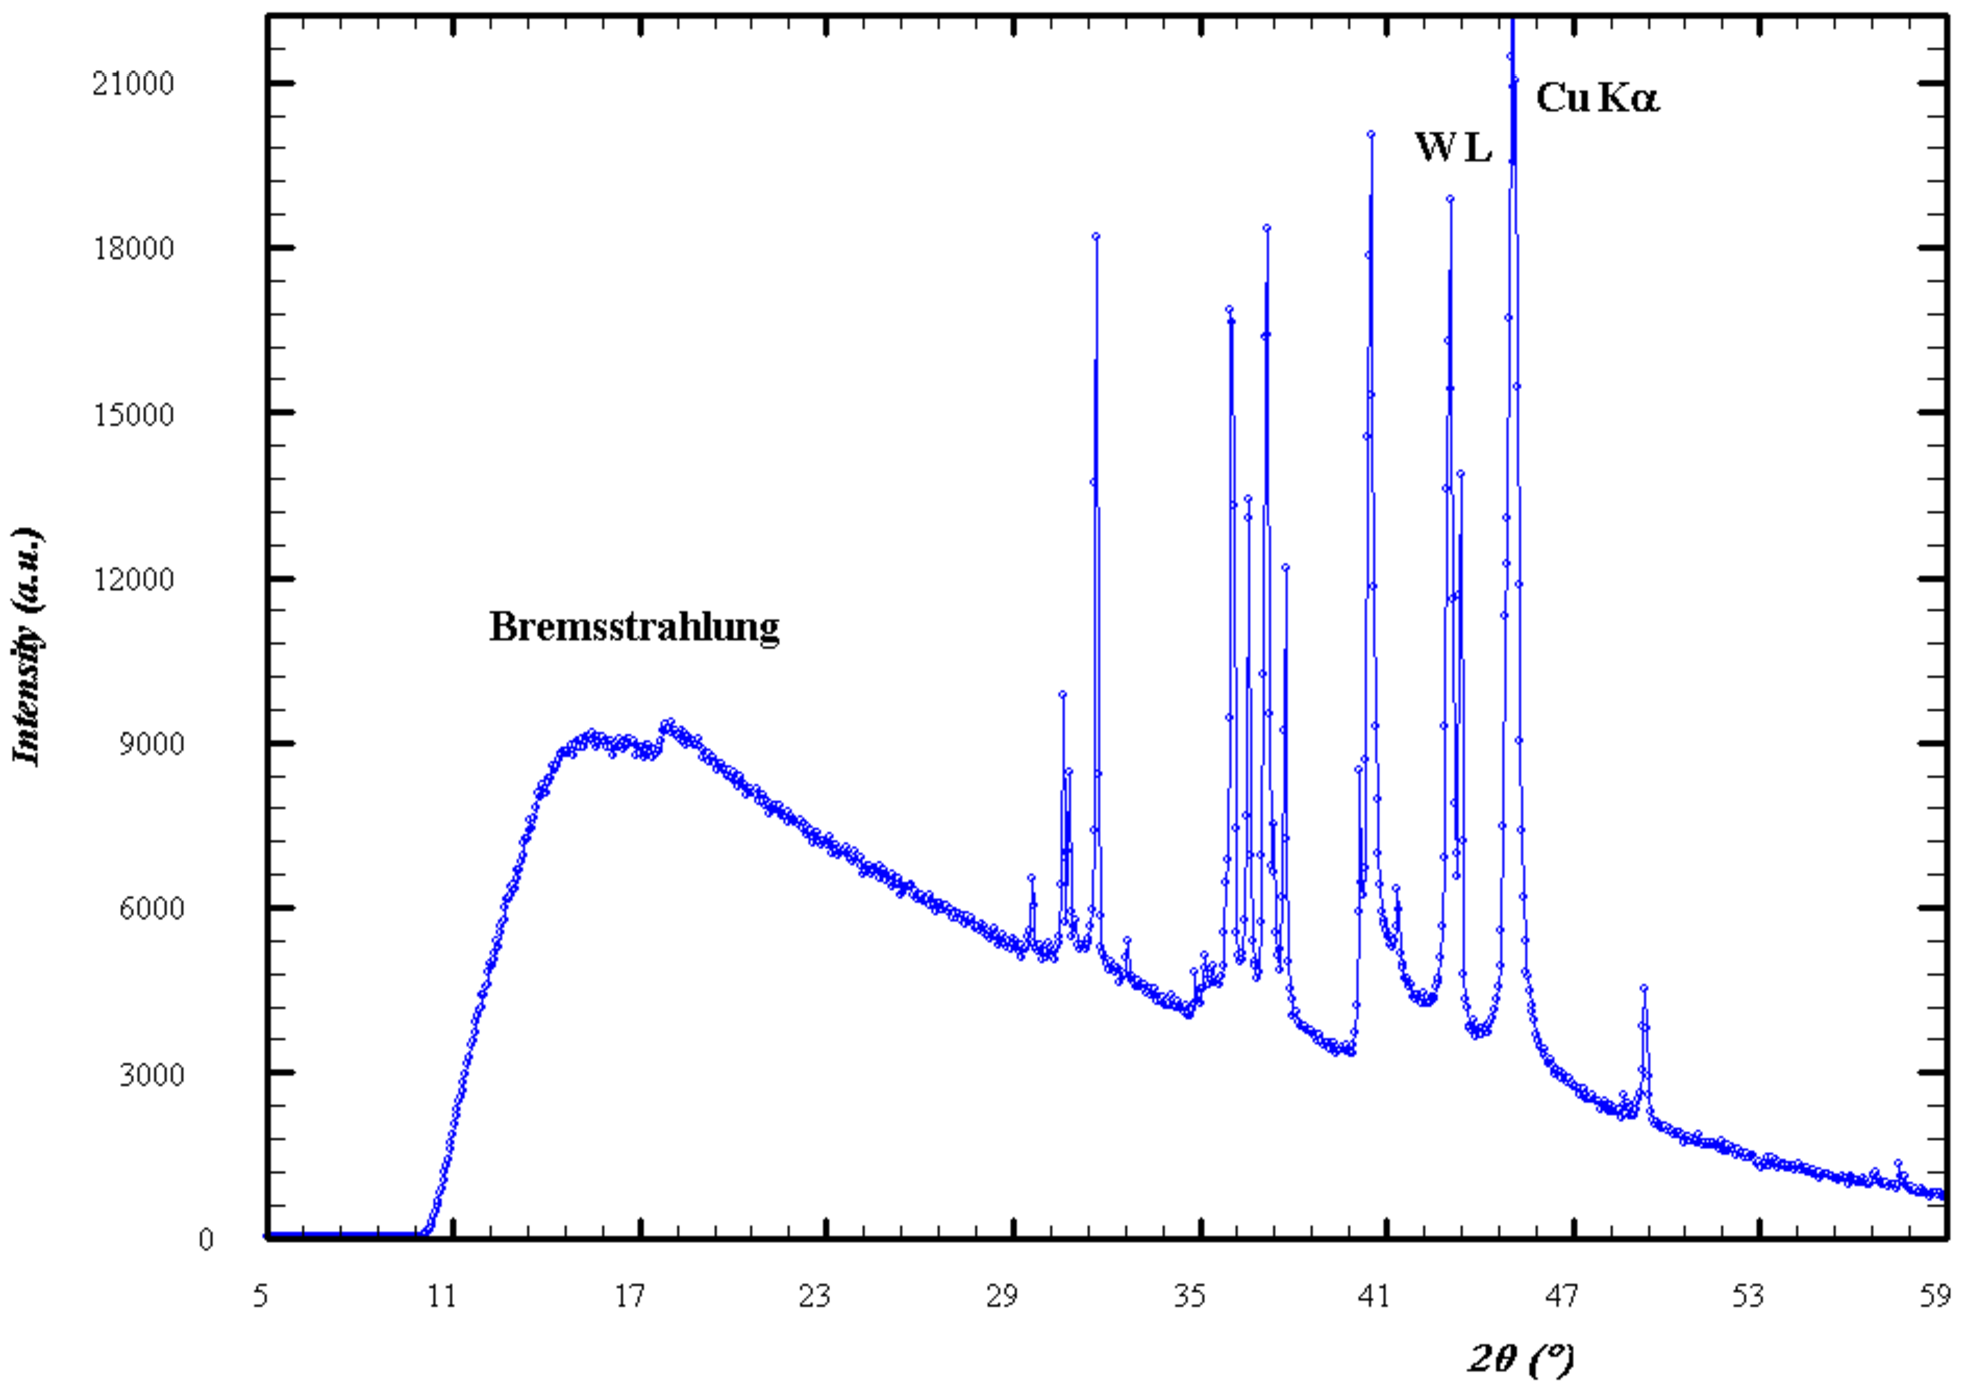
\includegraphics[width=1\textwidth]{./figures/Tube_Cu_LiF.pdf}
	\caption{Charakteristisches Spektrum einer Kupferanode nach Bragg-Reflexion an einem LiF-Kristall. Der Untergrund entsteht aufgrund der emittierten Bremsstrahlung der in der Anode gestreuten Elektronen. Auf diesem liegt das charakteristische Röntgenspektrum der Anode. Quelle: \url{http://commons.wikimedia.org/wiki/File:Tube_Cu_LiF.PNG} (Letzter Zugriff: 13. November 2014)}
	\label{fig:spektrum}
\end{figure}

Eine \textbf{Röntgenröhre} (schematisch in Abbildung \ref{fig:roehre}) besteht aus einem evakuierten Glaskolben mit einer Anordnung von geheizter Kathode und Anode aus Targetmaterial.
Zwischen Kathode und Anode wird die Beschleunigungsspannung $U$ angelegt, sodass beim Heizen der Kathode mit der Heizspannung $U_\mathrm{Heiz}$ aufgrund des glühelektrischen Effekts ein Teil der Elektronen die Austrittsarbeit der Kathode überwinden kann und durch die Beschleunigungsspannung $U$ in Richtung der Anode beschleunigt werden.
Nachdem die Beschleunigungsspannung $U$ durchlaufen wurde, treffen die Elektronen mit der Energie $e U$ auf das Anodenmaterial und erzeugen dabei Bremsstrahlung sowie charakteristische Strahlung, welche durch ein für Röntgenstrahlung durchlässiges Fenster im Glaskolben aus der Röhre austreten können.
\begin{figure}[h]
	\centering
	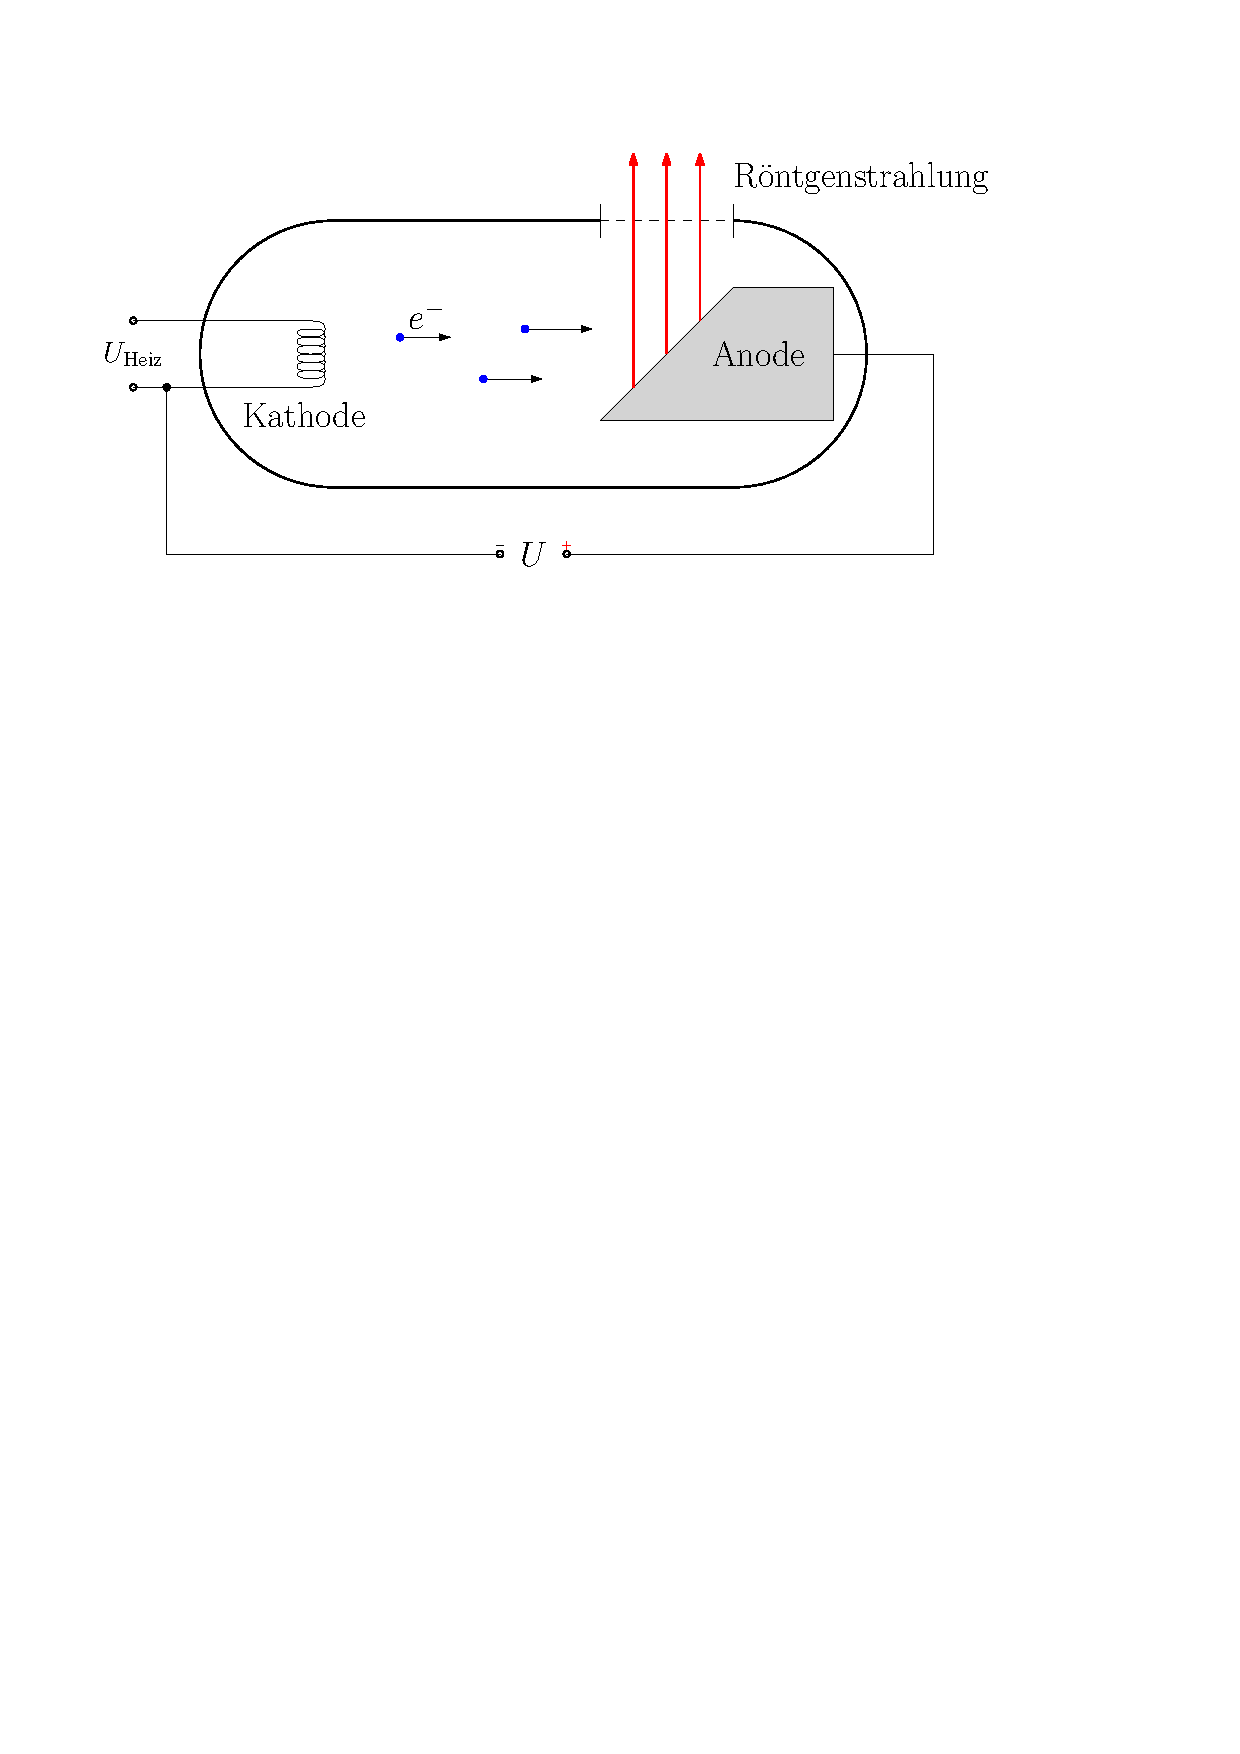
\includegraphics[width=0.75\textwidth]{./figures/roentgenroehre.pdf}
	\caption{schematischer Aufbau einer Röntgenröhre}
	\label{fig:roehre}
\end{figure}

\subsection{Röntgenstrahlung}

\subsubsection{Erzeugung und Nachweis}

\subsubsection{kontinuierliches und charakteristisches Röntgenspektrum}


\subsection{Geiger-Müller-Zählrohr}

\subsubsection{Aufbau}

\subsubsection{Funktionsweise}

\subsubsection{Totzeit und Totzeitkorrektur}


\subsection{Dosimetrische Messgrößen}

\subsubsection{Aktivität}
Zerfallsgesetz:
\begin{align}
	\frac{\mathrm{d} N(t)}{\mathrm{d} t} = - \lambda \cdot N(t)
\end{align}
beschreibt die Abnahme von Teilchen.
Aktivität beschreibt die Anzahl der Zerfälle pro Zeiteinheit also:
\begin{align}
	A(t) = - \frac{\mathrm{d} N(t)}{\mathrm{d} t} = \lambda \cdot N(t)
\end{align}

\subsubsection{Energiedosis}
Die im Absorberelement $\mathrm{d}V$ mit der Masse $\mathrm{d} m = \rho \cdot \mathrm{d}V$ deponierte Energie $\mathrm{d}E$:
\begin{align}
	D &= \frac{\mathrm{d}E}{\mathrm{d}m} = \frac{1}{\rho}\frac{\mathrm{d}E}{\mathrm{d}V}\\
	[D] &= \frac{\mathrm{J}}{\mathrm{kg}} = \mathrm{Gy} \quad \text{(Gray)}
\end{align}
Physikalische nicht biologische Größe.

\subsubsection{Ionendosis}
Bezeichnet die elektrische Ladung die durch ionisierende Strahlung in einer bestimmten Masse entsteht:
\begin{align}
	J = \frac{\mathrm{d}Q}{\mathrm{d}m}
\end{align}
Kann durch Kenntnis der mittleren Energie für die Bildung eines Ionenpaares in Energiedosis umgerechnet werden.

\subsubsection{Dosisleistung}
\begin{align}
	\dot{D} = \frac{\mathrm{d}D}{\mathrm{d}t}
\end{align}

\subsubsection{Äquivalentdosis}
Äquivalentdosis $H$.
Beachtet die relative biologische Wirksamkeit verschiedener Strahlungstypen durch Einführung eines Qualitätsfaktors $Q$.
\begin{align}
	H = Q \cdot D
\end{align}
Die Äquivalentdosis hat die gleiche Einheit wie die Dosis und wird daher um die physikalische Größe der Dosis von der Biologischen der Äquivalentdosis zu unterscheiden mit Sievert "beeinheitet".

Typische Qualitätsfaktoren (Gerthsen):
\begin{align*}
	&\text{Strahlungsart} \quad & Q / \si{Sv.Gy\tothe{-1}}\\
	&\text{Röntgen- und Gammastrahlung} \quad & 1 \\
	&\text{Betastrahlung} \quad & 1 \\
	&\text{Schnelle Neutronen} \quad & 10 \\
	&\text{Langsame Neutronen} \quad & 5 \\
	&\text{Alphastrahlung} \quad & 10 \\
	&\text{Schwere Rückstoßkerne} \quad & 20
\end{align*}


\subsection{Bildkontrast, Bildhelligkeit und visuelle Ortsauflösung}


\subsection{4-A Regel im Strahlenschutz}
\begin{itemize}
	\item \textbf{Abstand:}
	Die Wirkung von ionisierender Strahlung sinkt stark mit dem Abstand von der Quelle ($1/r^2$-Gesetz) und sollte daher stehts maximiert werden.
	Z.B. durch Sperrbereiche, ausgestrecktem Arm und andere Haltewerkzeuge (Zangen).
	
	
	\item \textbf{Aufenthaltszeit:}
	Die zugeführte Dosis ist proportional zur Aufenthaltszeit und sollte damit minimiert werden.
	
	
	\item \textbf{Abschirmung:}
	Durch geeignete Abschirmung kommt es zu einem exponentiellen Abfall der Strahlungsintensität im Absorber (Lambert-Beer-Gesetz).
		
	
	\item \textbf{Aktivität:}
	Die Aktivität eines Präparats sollte bekannt sein und wenn möglich minimiert werden.
	D.h. wenn es das Experiment erlaubt sollte ein Präparat geringerer Aktivität verwendet werden.
	
	
\end{itemize}


\subsection{Aufbau und Funktionsweise verschiedener Personendosimeter}


\subsection{Abschwächung von Röntgenstrahlen (Lambertsches Schwächungsgesetz)}


\section{Versuchsaufbau}

\section{Durchführung und Auswertung}

Die ausführliche Durchführung ist der Versuchsanleitung \cite{anleitung} zu entnehmen.
Sollten Abweichungen bei der Durchführung auftreten, so werden diese im jeweiligen Unterkapitel dargestellt.
\section{Fazit}

\FloatBarrier
% BIBLIOGRAPHIE
\vspace{\fill}
% Maximale Anzahl der Einträge in Klammer
% Zitieren mit \cite{lamport94}
\begin{thebibliography}{19}
\bibitem{siegbahn}
	K. Siegbahn,
	\emph{Alpha-, Beta- and Gamma-Ray Spectroscopy},
	Elsevier Science Ltd. 1965

\bibitem{anleitung}
	Physikalisches Praktikum V: Kern- und Teilchenphysik,
	Versuchsbeschreibung \emph{P523: $\beta$-Spektrometer} (Stand: Januar 2015),
	Universität Bonn	

\bibitem{riezler}
	Riezler, W.; Kopitzki, K.
	\emph{Kernphysikalisches Praktikum},
	Teubner 1963

\bibitem{nist}
	M. P. Unterweger, D. D. Hoppes, F. J. Schima, J.S. Coursey,
	\emph{NIST Radionuclide Half-Life Measurements},
	\url{http://www.nist.gov/pml/data/halflife-html.cfm} (Letzter Abruf: 1. Mai 2015)

\end{thebibliography}

% APPENDIX
\begin{appendix}
\section{Anhang}

\end{appendix}

\end{document}
